\documentclass[11pt]{article}
\usepackage[margin=22mm]{geometry}
\usepackage{tikz}
\usepackage{pgfplots}
\usepackage{luanumbers}

\pgfplotsset{compat=1.18}
\LuaNumbersSetup{decimals=1,warnings=error}

\begin{document}
Outside graphics, 3.14159 is rounded.

% Geometry is protected; only the explicit \LuaNumber call is rounded.
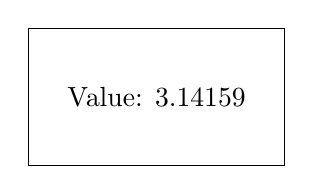
\begin{tikzpicture}[x=1.00cm,y=1.00cm]
  \draw (0.00,0.00) rectangle (3.26,1.74);
  \node at (1.63,0.87) {Value: \LuaNumber{3.14159}};
\end{tikzpicture}

% Plot coordinates remain exact. PGFPlots controls generated tick labels.
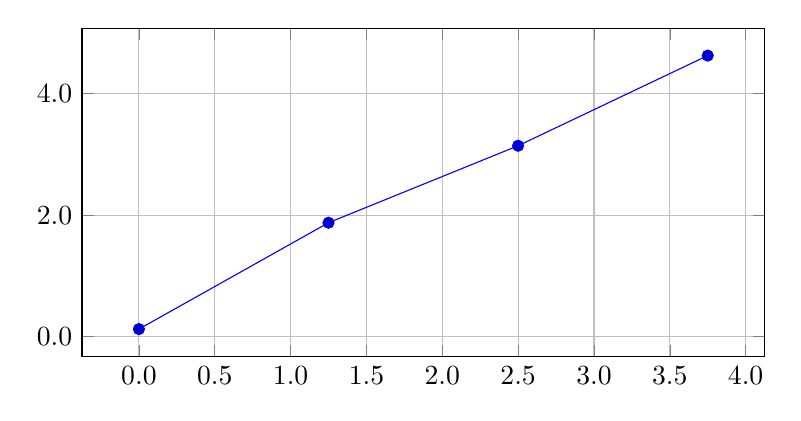
\begin{tikzpicture}
  \begin{axis}[
    width=10.25cm,
    height=5.75cm,
    grid=major,
    tick label style={/pgf/number format/.cd,
      fixed,fixed zerofill,precision=1}
  ]
    \addplot coordinates {
      (0.00,0.125) (1.25,1.875) (2.50,3.14159) (3.75,4.625)
    };
  \end{axis}
\end{tikzpicture}
\end{document}
